
El momento de un mu\'on \textit{low-$p_{T}$} es extraido a partir de la reconstrucci\'on de su trayectoria a trav\'es de las se\~nales que deja en el tracker junto con los impactos en el sistema de muones mediante un ajuste por filtro de Kalman~\cite{Kalman1960ANA}. \\

En el caso de muones \textit{high-$p_{T}$}, part\'iculas adicionales generadas en las cascadas electromagn\'eticas dejan t\'ipicamente impactos y segmentos adicionales en las distintas c\'amaras, provocando que estas se\~nales adicionales sean probablemente utilizadas en el ajuste por filtro de Kalman en lugar de las se\~nales que realmente provienen del mu\'on que se quiere medir, o equivalentemente, un n\'umero elevado de impactos en una c\'amara en particular puede dificultar seriamente la propia reconstrucci\'on. Es por esto que los muones de alto momento requieren un tratamiento m\'as cuidadoso de la informaci\'on encontrada en el sistema de muones, lo que se conoce como reajustes, que seleccionan qu\'e impactos van a utilizarse en el proceso de reconstrucci\'on de la traza y cu\'ales no. \\

En las siguientes subsecciones se da una descripci\'on general de los distintos reajustes para muones \textit{high-$p_{T}$} que actualmente se llevan a cabo en CMS, as\'i como del algoritmo utilizado para la asignaci\'on final del momento transverso.

\subsection{Reajuste TPFMS (\textit{Tracker-plus-first-muon-station})}\label{sec:TPFMS}

El primer reajuste, que es el m\'as sencillo en cuanto a su implementaci\'on, es el TPFMS, que selecciona \'unicamente las se\~nales en el tracker y en la estaci\'on m\'as interna del sistema de muones que contiene impactos. De esta manera se pretende desechar aquellos impactos de estaciones m\'as lejanas y eleminar as\'i la posible contaminaci\'on proveniente de las cascadas electromagn\'eticas.

\subsection{Reajuste Picky}\label{sec:Picky}

El reajuste Picky tiene como objetivo encontrar posibles cascadas y eliminar sus se\~nales adicionales del ajuste de la traza. De esta manera, si m\'as de $n$ impactos se encuentran dentro de un cono en torno a un impacto concreto, la estaci\'on en la que se encuentran dichas se\~nales se marca como contaminada. As\'i, a la hora de hacer el ajuste a la traza, si su $\chi$\textsuperscript{2} est\'a por encima de un cierto umbral, se eliminan del mismo aquellos impactos que se encuentren en c\'amaras contaminadas y se repite el ajuste de nuevo. \\
Los par\'ametros del algoritmo $n$ y $\chi$ est\'an optimizados en base a estudios sobre simulaciones.

\subsection{Reajuste DYT (\textit{Dynamic truncation})}\label{sec:DYT}

Cuando un mu\'on pierde una gran fracci\'on de su energ\'ia durante su trayecto, su direcci\'on puede cambiar y las se\~nales encontradas en las siguientes estaciones pueden ser inconsistentes con la trayectoria inicial (ver Figura~\ref{fig:energyloss}), provocando problemas a la hora de reconstruir la traza y consecuentemente al tratar de asignar un valor acertado a su momento transverso. En estos casos, el reajuste DYT considera m\'as conveniente parar el filtro de Kalman una vez que un cambio en la trayectoria del mu\'on es detectado. \\
En el reajuste DYT se define un operador $E$ que da idea de la compatibilidad de un determinado segmento en una c\'amara con la extrolaci\'on de la traza interna a dicha c\'amara, de manera que si este operador supera un valor predeterminado, el filtro de Kalman se detiene y no tiene en cuenta aquellos impactos en las c\'amaras posteriores al cambio de trayectoria detectado. 

\begin{figure}[h]
\centering
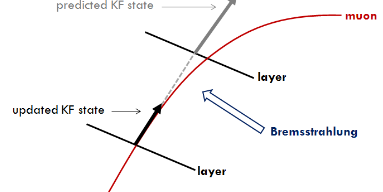
\includegraphics[width=0.60\textwidth]{figures/energyloss.png}
\caption{Representaci\'on gr\'afica del cambio en la trayectoria del mu\'on tras una gran p\'erdida de energ\'ia por Bremsstrahlung.}
\label{fig:energyloss}        
\end{figure}


\subsection{Asignaci\'on final de momento transverso: el algoritmo TuneP}\label{sec:TuneP}

Finalmente, la recomendaci\'on central de la colaboraci\'on CMS para la asignaci\'on del momento transverso de los muones \textit{high-$p_{T}$} se corresponde con el proporcionado por el algoritmo TuneP. \\
 El objetivo de este algoritmo es simplemente eligir cu\'al es la mejor reconstrucci\'on de la traza posible de entre la traza reconstruida \'unicamente en el tracker y las trazas obtenidas por los distintos reajustes (TPFMS, Picky y DYT). Dicha elecci\'on se hace teniendo en cuenta conjuntamente el $\chi$\textsuperscript{2}/ndof y el $\sigma_{p_{T}}/p_{T}$ de las trazas consideradas.
